\chapter{Aplicação 2: Epidemia de Ebola na África Ocidental}\label{chap:ebola}


Em meados de março de 2014 os primeiros casos de Ebola foram detectados na Guiné, e futuras investigações epidemiológicas iriam sugerir que os primeiros casos ocorreram por volta de Dezembro de 2013. Em março de 2016, já se somavam 28.816 suspeitas, possibilidades e casos confirmados de Ebola em Guiné, Libéria e Serra Leoa, com 11.310 mortes. Isso marca a epidemia de Ebola do período de 2013-2016 como uma das piores na história \cite{Carvalho2019}. Isso pois o Ebola já tem casos registrados desde 1976, o primeiro deles na República Democrática do Congo. A pergunta científica que se faz então é: quais foram os fatores relevantes para o considerável aumento repentino do número de casos e de sua propagação geográfica. Para isso, vamos utilizar as técnicas desenvolvidas ao longo do texto para lidar com este problema. 

Seguindo os estudos de \cite{Carvalho2019}, um rico conjunto de dados socioeconômicos, climáticos e genéticos foi disponibilizado. Os dados vem agregados em área para os distritos da Serra Leoa, prefeituras da Guiné e condados da Libéria. Das 81 localidades resultantes, 63 reportaram 1 ou mais casos de Ebola. Essas regiões estão dispostas na \autoref{fig: mapa_ebola}.

\begin{figure}[h]
    \centering
    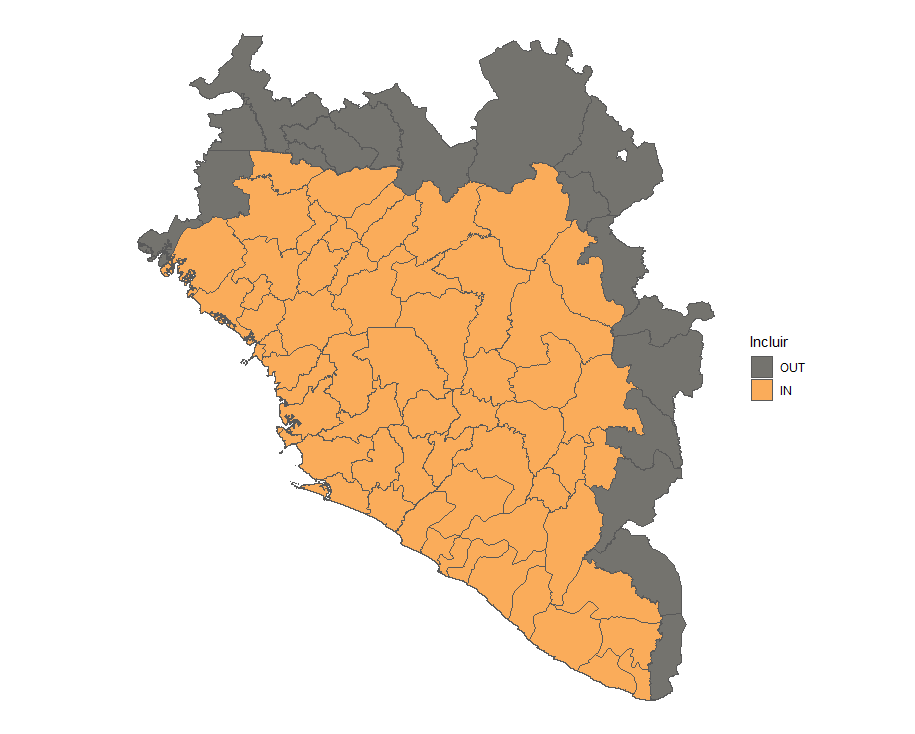
\includegraphics[width = 0.8\linewidth]{images/ebola_regions.png}
    \caption{Regiões da África Ocidental consideradas no modelo. Regiões com a marcação IN registraram 1 ou mais casos de Ebola. }
    \label{fig: mapa_ebola}
\end{figure}

 Os preditores utilizados estão disponíveis na \autoref{tab:ebola_predictors}. 

\begin{figure}
    \centering
    \begin{minipage}{0.45\textwidth}
        \centering
        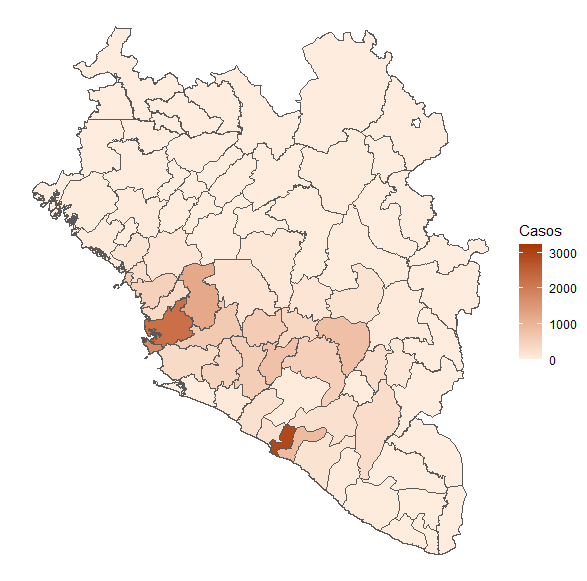
\includegraphics[width=0.9\textwidth]{images/raw_cases_ebola.png} % first figure itself
        \caption{Mapa dos casos brutos de ebola.}
    \end{minipage}\hfill
    \begin{minipage}{0.45\textwidth}
        \centering
        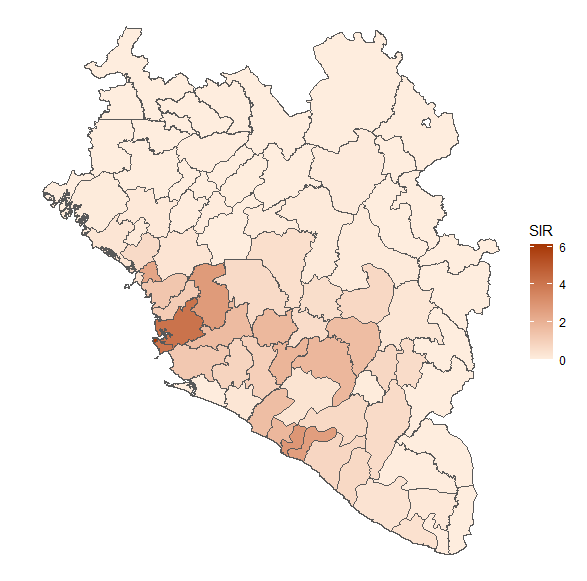
\includegraphics[width=0.9\textwidth]{images/SIR_ebola.png} % second figure itself
        \caption{Mapa da SIR para o caso do Ebola. A população suscetível foi considerada a população total.}
    \end{minipage}
\end{figure}

\begin{table}[h]
    \centering
    \begin{tabular}{|p{5cm} |p{5cm} |p{5cm} |}
    \hline
        Tipo de preditor & Abreviação & Descrição \\ \hline
        Demográfico & pdensMN & Densidade populacional (hab/km$^2$) \\\hline
       Demográfico &geconMN& Produção econômica média\\\hline
        Demográfico&geconMIN& Mínimo da produção econômica\\\hline
        Demográfico&geconMAX& Máximo da produção econômica\\\hline
        Demográfico&geconSTD& Desvio padrão da produção econômica\\\hline
        Demográfico&ttXkMN& Tempo de viagem média estimado para a cidade mais próxima com uma população de pelo menos $X \times 10.000$ habitantes, para $X = 50, 100$ e $500$\\\hline
        Climático&altMN& Altitude média\\\hline
        Climático&tempMN& Temperatura anual média\\\hline
        Climático&tempssMN&Sazonalidade média da temperatura\\\hline
        Climático&precMN& Precipitação anual média\\\hline
        Climático&precssMN&Sazonalidade média da precipitação \\\hline
        Filogenético&Introadmin& Número médio de introduções virais preditas usando fronteiras administrativas\\\hline
        Filogenético&Introdista& Número médio de introduções virais preditas usando fronteiras administrativas\\
        \hline
    \end{tabular}
    \caption{Preditores considerados para a modelagem da epidemia de Ebola. Todos os preditores contínuos foram padronizados subtraindo-se a média e dividindo pelo desvio-padrão.}
    \label{tab:ebola_predictors}
\end{table}


Para a modelar a contagem de casos utilizarei 6 modelos diferentes: Poisson Log-normal simples, Poisson Log-normal com ORLE e o modelo BYM2, e todos estes modelos novamente mas com a inclusão do esquema de seleção de variáveis SSVS de Kuo e Mallick. Para cada modelo também teremos o WAIC como comparativo, a eficiência em (ESS/s) e o erro médio quadrático à posteriori, disposta na \autoref{tab:posterior_summary_ebola}. Foi rodada uma única cadeia com 300.000 iterações, 200.000 de \textit{burnin} com parâmetro de thinning igual a 10 para cada modelo.

Os diagnósticos de cadeia não foram muito satisfatórios. A quantidade de amostras efetivas produzidas por rodada é bem baixa. Os parâmetros $\beta$ apresentaram alta autocorrelação, o que sinaliza convergência lenta. Apesar disso, os resultados em termos de WAIC e RMSE foram bons. Antes de comparara relevância das variáveis, um resultado interessante apresentado foi o BYM2 no cenário de seleção de variáveis. Aplicando o teste de Moran para cada covariável, apenas uma não apresenta forte estrutura espacial que foi a de densidade populacional. Todas as outras tiveram p-valor menor que 0.0001. O BYM2 acabou absorvendo toda a informação espacial, e nenhuma variável foi selecionada mais de 20 \% das vezes. No modelo com a inclusão de todas as variáveis o parâmetro $\rho$ se comportou de forma parecida com a priori uniforme, comportamento similar aos testes da \autoref{sec:spatial} de quando não havia resíduo espacial. Na seleção de variáveis, a média a posteriori de $\rho$ salta para 0.8, indicando forte associação espacial, e nenhuma variável foi selecionada. 

Por este motivo, utilizarei o modelo com ORLE para analisar a relevância de variáveis. Um ponto a se notar aqui é a alta correlação entre as covariáveis (\autoref{fig:corplot}), que afeta a interpretação dos resultados. outro problema está na convergência: a cadeia visita o espaço de modelos de forma bem lenta. A tendência observada foi de terem variáveis que sempre são selecionadas, e as outras variáveis sendo selecionadas esporadicamente. A cadeia consegue se desvencilhar do estado inicial. Para avaliar a situação melhor, rodei 400 cadeias em paralelo, observando as frequências de modelo escolhidas em cada uma. As cadeias começam todas de pontos diferentes: 100 delas começando de $\gamma = (0,\dots, 0)$, 100 delas começando em $\gamma = (1, \dots, 1)$, e o resto de algum ponto aleatório uniformemente escolhido em $\{0,1\}^p$. Apresento como resultado as médias à posteriori da indicadora de cada covariável:

\begin{table}[]
    \centering
    \begin{tabular}{|c|c|}
    \hline
            \textbf{Covariável}& \textbf{Média} \\ \hline
            geconMN  & 0.09  \\ \hline
            geconMIN  & 0.36  \\ \hline
            geconMAX  & 0.14  \\ \hline
            geconSTD  & 0.04  \\ \hline
            pdensMN  & 0.07  \\ \hline
            tt50kMN  & 0.20  \\ \hline
            tt100kMN  & 0.38  \\ \hline
            tt500kMN  & 0.18  \\ \hline
            altMN  & 0.21  \\ \hline
            tempMN & 0.33  \\ \hline
            tmpssMN & 0.42 \\ \hline
            precMN & 0.16 \\ \hline
            precssMN & 0.56  \\ \hline
            Introadmin & 0.04  \\ \hline
            Introdista & 0.03 \\ \hline
    \end{tabular}
    \caption{Médias \textit{à posteriori} das indicadoras das covariáveis para as múltiplas cadeias do modelo com ORLE.}
    \label{tab:posterior_gamma}
\end{table}



As análises do fator de Bayes não serão interessantes nesse cenário de fraca convergência da cadeia. Mas podemos gerar mapas da probabilidade \textit{à posteriori} da SIR ser maior do que 1, assim como realizar a predição das regiões sem casos. Aqui o modelo BYM2 mostra sua vantagem em relação ao BYM. A posteriori para $\tau_b$ é compatível com ambos os grafos de adjacências. Os resultados estão dispostos na \autoref{fig:pred}

\begin{figure}
    \centering
    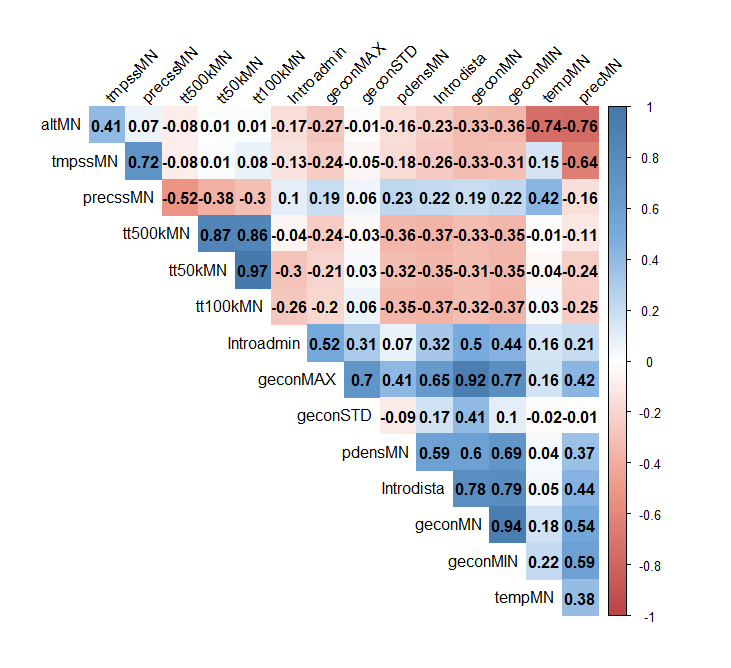
\includegraphics[width = 0.5\linewidth]{images/correlation_btwn_cov_ebola.png}
    \caption{Correlação entre as variáveis disponíveis para o estudo do Ebola. Destas, apenas a densidade populacional (pdensMN) não apresenta forte estrutura espacial.}
    \label{fig:corplot}
\end{figure}


\begin{table}
\centering
\begin{tabular}{@{}lrrcrrcccc@{}}\toprule
& SSVS & \phantom{ab}&  WAIC & \phantom{ab}& Eficiência & \phantom{ab}& Eficiência mínima & \phantom{ab}& RMSE\\

%\cmidrule{2-3} \cmidrule{5-6}
%& $Média$ & $(upp,lwr)$ && $Média$ & $(upp,lwr)$\\
\midrule
\textbf{Simples} & Não &&  5856.5 && 126.2 &&  30.4 && 139.9\\ 
\textbf{ORLE} & Não &&  459.7 && 145.1  &&  0.03 && 0.68\\ 
\textbf{BYM2} & Não &&  699.4 && 30.25  && 0.03 && 0.77\\
\textbf{Simples} & Sim &&  5670.6 && 6.26 && 0.165 && 141.0\\  
\textbf{ORLE} & Sim &&  475.5  &&  37.0 && 0.01  && 0.72\\ 
% var.s  0.6504600  0.6433667 0.1170732  0.4446273  0.90150079
\textbf{BYM2} & Sim &&  711.9 && 39.05 && 0.01 && 1.24\\

\bottomrule
\end{tabular}
    \caption{Comparativo dos 6 modelos usados para modelagem dos casos de Ebola. Eficiência (ESS por segundo) representa a eficiência média de todos os parâmetros da cadeia. Eficiência mínima é a menor eficiência encontrada. RMSE é a raiz do Erro Médio Quadrático.}
    \label{tab:posterior_summary_ebola}
\end{table}


\begin{figure} % "[t!]" placement specifier just for this example
\begin{subfigure}{0.38\textwidth}
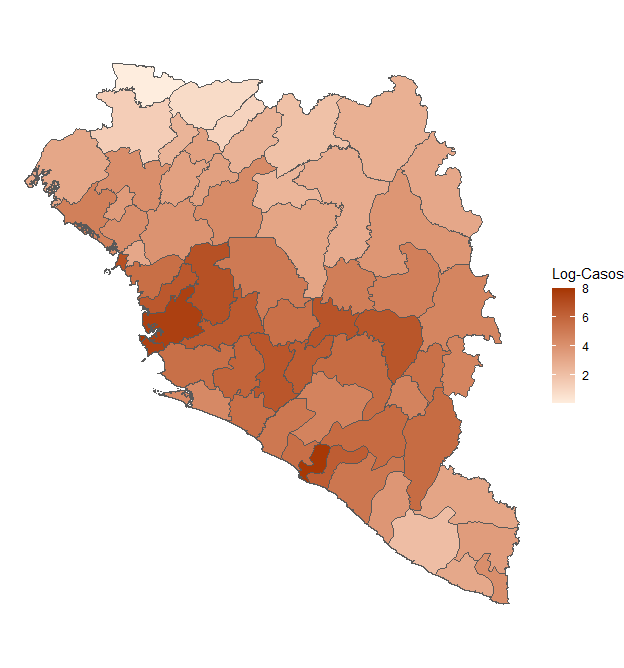
\includegraphics[width=\linewidth]{images/posterior_mean_simples.png}
\caption{Modelo simples} \label{fig:a}
\end{subfigure}\hspace*{\fill}
\begin{subfigure}{0.38\textwidth}
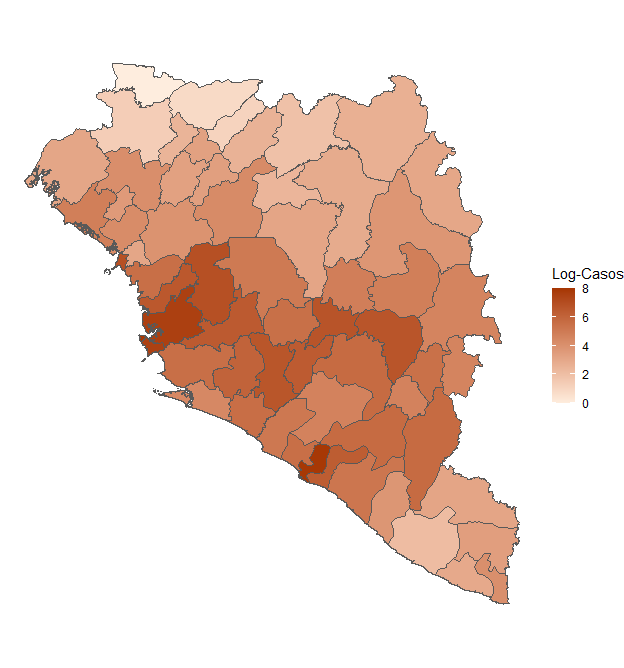
\includegraphics[width=\linewidth]{images/posterior_mean_ssvs.png}
\caption{Modelo simples com seleção de variáveis} \label{fig:b}
\end{subfigure}

\medskip
\begin{subfigure}{0.38\textwidth}
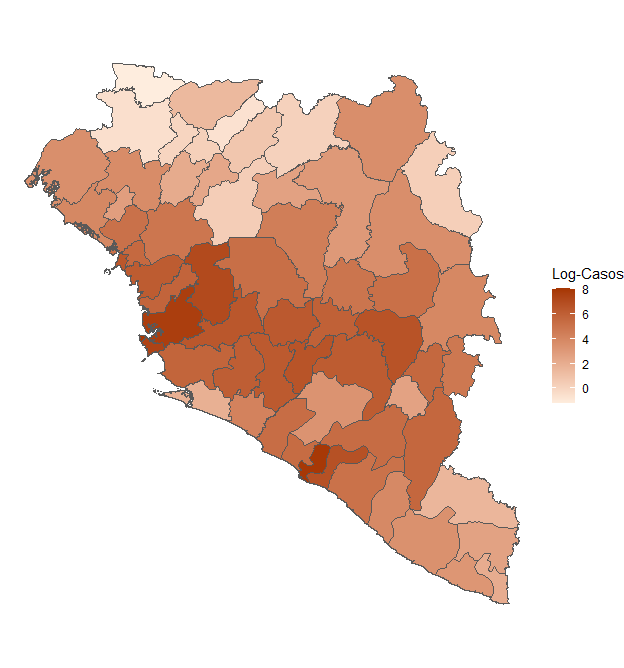
\includegraphics[width=\linewidth]{images/posterior_mean_orle.png}
\caption{Modelo com ORLE} \label{fig:c}
\end{subfigure}\hspace*{\fill}
\begin{subfigure}{0.38\textwidth}
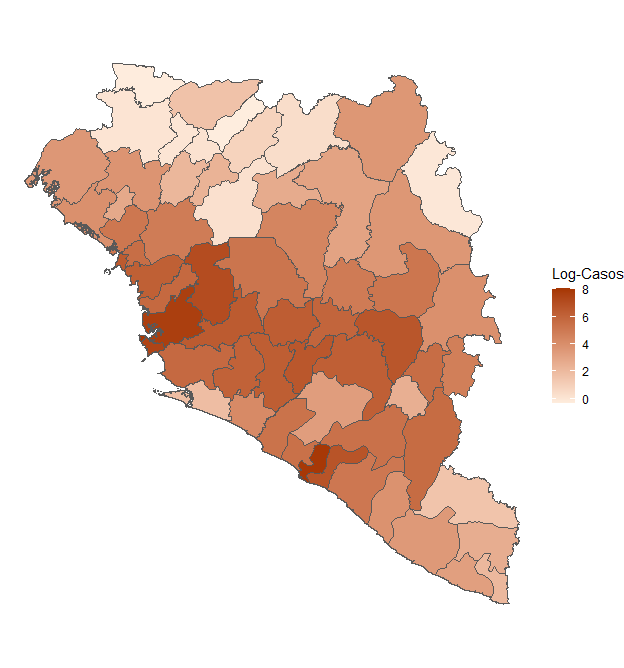
\includegraphics[width=\linewidth]{images/posterior_mean_orle_ssvs.png}
\caption{Modelo com ORLE e seleção de variáveis} \label{fig:d}
\end{subfigure}

\medskip
\begin{subfigure}{0.38\textwidth}
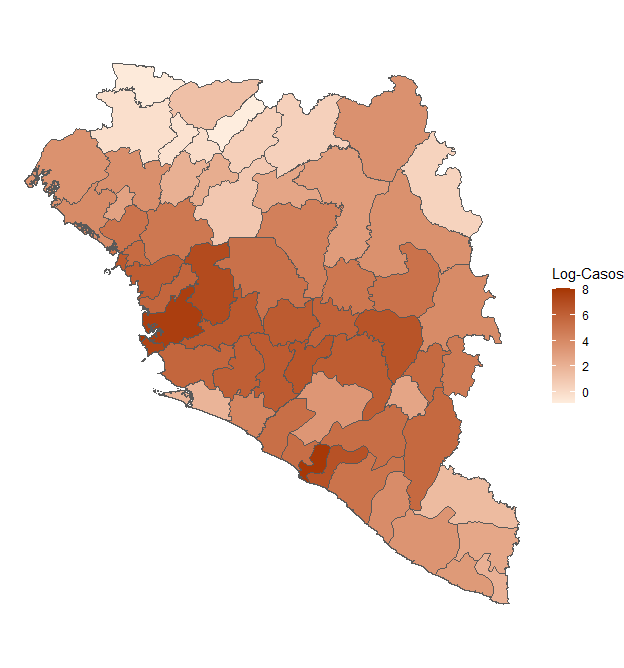
\includegraphics[width=\linewidth]{images/posterior_mean_bym2.png}
\caption{Modelo BYM2} \label{fig:e}
\end{subfigure}\hspace*{\fill}
\begin{subfigure}{0.38\textwidth}
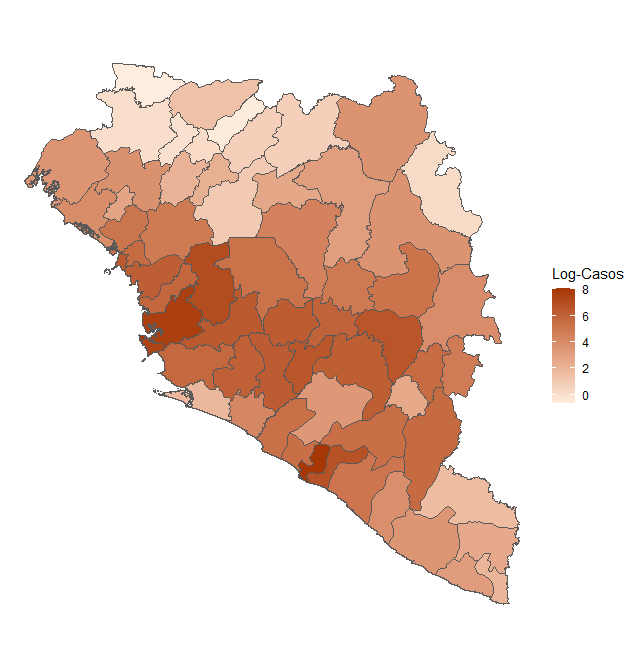
\includegraphics[width=\linewidth]{images/posterior_mean_bym2_ssvs.png}
\caption{Modelo BYM2 com seleção de variáveis} \label{fig:f}
\end{subfigure}

\caption{Mapa do log da média a posteriori de casos para os seis modelos de contagem de casos utilizados} \label{fig:ebola_posterior_maps}
\end{figure}

\begin{figure}
    \centering
    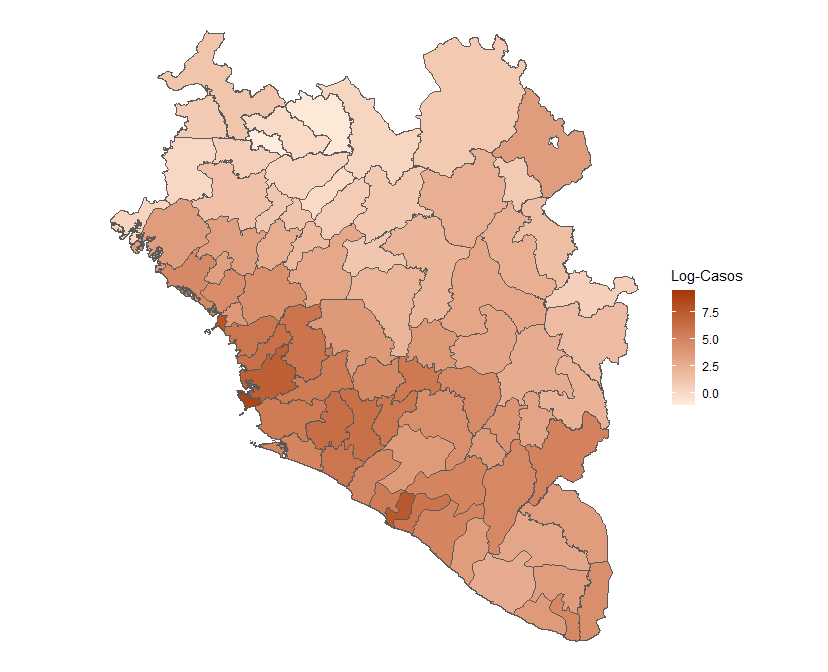
\includegraphics[width = 0.8\linewidth]{images/posterior_predicitve_bym2.png}
    \caption{Preditiva à posteriori, incluindo regiões agora que não tiveram casos registrados.}
    \label{fig:pred}
\end{figure}